\documentclass{article}
\usepackage[utf8]{inputenc}
\usepackage{amsmath}
\usepackage{tikz}

\newcommand\scalemath[2]{\scalebox{#1}{\mbox{\ensuremath{\displaystyle #2}}}}

\begin{document}
	
	Temos o problema de contorno definido por, para $ (x, y) \in (0, 1)^2 $ , \\
	\begin{gather}
		-\nabla(\kappa\nabla T) = 0 \texttt{;} \\
		T(x, 0) = T(x, 1) = a \texttt{;} \\
		T(0, y) = b \texttt{;} \, -\kappa \frac{\partial T}{\partial x}(1, y) = h(T - T_{\text{out}})\texttt{.}
	\end{gather}

	
	Consider the boundary conditions:
	\begin{align*}
		T(x, 1) &= a \\
		T(0, y) &= b \\
		-\kappa \frac{\partial T}{\partial x}(1, y) &= h(T - T_{\text{out}})
	\end{align*}
	
	\begin{tikzpicture}
		\draw[step=1cm,gray,very thin] (0,0) grid (3,4);
		\draw[thick] (0,0) -- (0,4) -- (3,4) -- (3,0) -- cycle;
		
		\node at (-0.5, 1.5) {$b$};
		\node at (1.5, 4.5) {$a$};
		\node at (1.5, -0.5) {$a$};
		\node at (4.8, 2.5) {$-\kappa \frac{\partial T}{\partial x} = h(T - T_{\text{out}})$};
	\end{tikzpicture}

	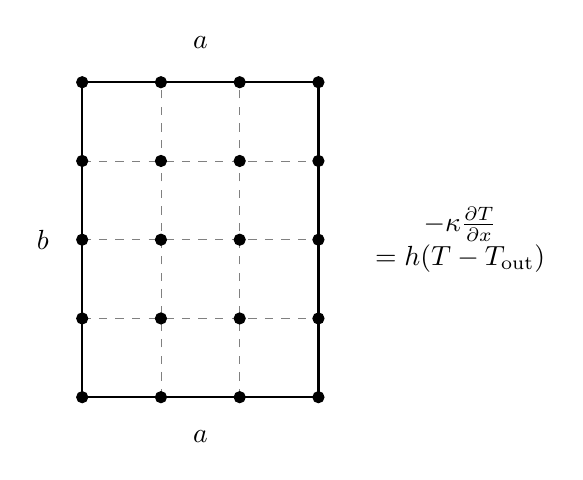
\begin{tikzpicture}
		% Draw a 3x4 grid with dashed lines
		\draw[step=1cm,gray,very thin, dashed] (0,0) grid (3,4);
		
		% Draw the boundary of the grid
		\draw[thick] (0,0) -- (0,4) -- (3,4) -- (3,0) -- cycle;
		
		% Place dots at each intersection of the grid
		\foreach \x in {0,1,2,3}
		\foreach \y in {0,1,2,3,4}
		\filldraw[black] (\x,\y) circle (2pt);
		
		% Add labels next to the grid
		\node at (-0.5, 2) {$b$};
		\node at (1.5, 4.5) {$a$};
		\node at (1.5, -0.5) {$a$};
		\node[align=center] at (4.8, 2) {$-\kappa \frac{\partial T}{\partial x}$ \\ $= h(T - T_{\text{out}})$};
	\end{tikzpicture}
	
	
	\begin{align*}
		-\nabla^2 u(x, y) &= f(x, y), && \text{(PDE)}\\
		u(x, 0) &= g_1(x), && \text{(Dirichlet condition at }y=0)\\
		u(x, h) &= g_2(x), && \text{(Neumann condition at }y=h)\\
		-\frac{\partial u}{\partial y}(x, 0) &= h_1(x), && \text{(Neumann condition at }y=0)\\
		\frac{\partial u}{\partial y}(x, h) &= h_2(x), && \text{(Dirichlet condition at }y=h)
	\end{align*}
	
	
	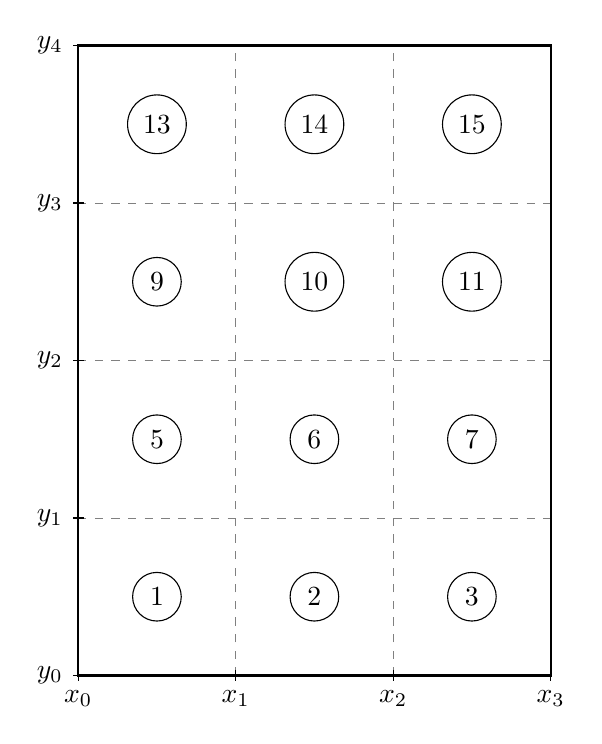
\begin{tikzpicture}[scale=2, every node/.style={scale=1}]
		
		% Draw the grid with dashed lines
		\draw[step=1cm,gray,very thin, dashed] (0,0) grid (3,4);
		
		% Draw the solid lines around the grid
		\draw[thick] (0,0) rectangle (3,4);
		
		% Label the x coordinates
		\foreach \x in {0,...,3} 
		\draw (\x cm,1pt) -- (\x cm,-1pt) node[anchor=north] {$x_{\x}$};
		
		% Label the y coordinates
		\foreach \y in {0,...,4} 
		\draw (1pt,\y cm) -- (-1pt,\y cm) node[anchor=east] {$y_{\y}$};
		
		% Place the nodes and label them
		\foreach \y in {1,...,4}
		\foreach \x in {1,...,3}
		\node[circle, draw, fill=white] at (\x-0.5,\y-0.5) {\pgfmathparse{int((\y-1)*4+\x)}\pgfmathresult};
		
	\end{tikzpicture}
	
	
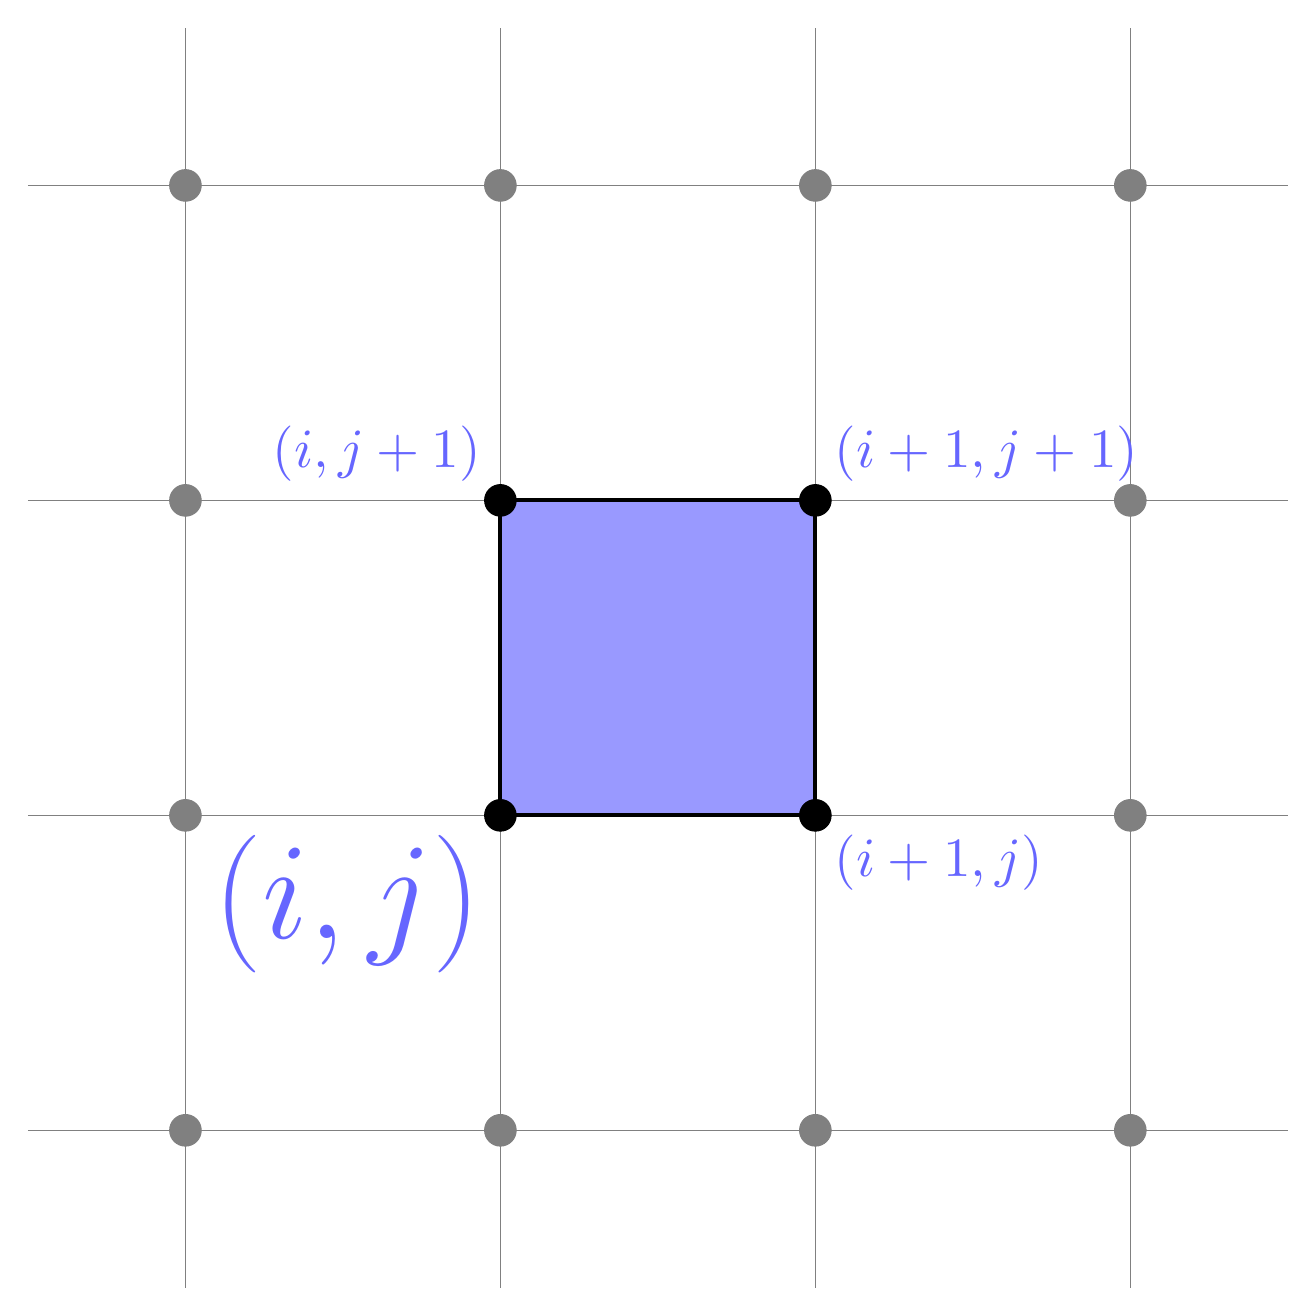
\begin{tikzpicture}[scale=2, every node/.style={scale=2}]
	
	
	\draw [style=help lines, step=2]                (-1,-1)    grid        (+7,+7);
	\draw [line width=0.5mm, fill=blue!40!white]    (+2,+2)    rectangle    (+4,+4);
	
	\draw [blue!60!white] (  2,  2) node[anchor=north east] {\Huge $(i  ,j  )$};
	\draw [blue!60!white] (  4,  2) node[anchor=north west] {$(i+1,j  )$};
	\draw [blue!60!white] (  4,  4) node[anchor=south west] {$(i+1,j+1)$};
	\draw [blue!60!white] (  2,  4) node[anchor=south east] {$(i  ,j+1)$};
	
	\filldraw [color=gray]    (0,0) circle (.1);
	\filldraw [color=gray]    (0,2) circle (.1);
	\filldraw [color=gray]    (0,4) circle (.1);
	\filldraw [color=gray]    (0,6) circle (.1);
	\filldraw [color=gray]    (2,0) circle (.1);
	\filldraw [color=black]    (2,2) circle (.1);
	\filldraw [color=black]    (2,4) circle (.1);
	\filldraw [color=gray]    (2,6) circle (.1);
	\filldraw [color=gray]    (4,0) circle (.1);
	\filldraw [color=black]    (4,2) circle (.1);
	\filldraw [color=black]    (4,4) circle (.1);
	\filldraw [color=gray]    (4,6) circle (.1);
	\filldraw [color=gray]    (6,0) circle (.1);
	\filldraw [color=gray]    (6,2) circle (.1);
	\filldraw [color=gray]    (6,4) circle (.1);
	\filldraw [color=gray]    (6,6) circle (.1);
	
\end{tikzpicture}	


Let $\alpha_x$, $\alpha_y$, and $\beta$ be given constants, and $a$, $b$, and $T_{\text{out}}$ be given boundary conditions. Then the linear system $AT = b$ for the given equations can be written as:

\begin{equation}\scalemath{0.5}{
A = \begin{bmatrix}
	-2(\alpha_x + \alpha_y) & \alpha_x            & 0                   & \alpha_y            & 0                   & 0                   & 0                   & 0                   & 0 \\
	\alpha_x               & -2(\alpha_x + \alpha_y) & \alpha_x            & 0                   & \alpha_y            & 0                   & 0                   & 0                   & 0 \\
	0                   & \alpha_x            & -(2\alpha_x (1 + \beta/2) + 2\alpha_y) & 0                   & 0                   & \alpha_y            & 0                   & 0                   & 0 \\
	\alpha_y               & 0                   & 0                   & -2(\alpha_x + \alpha_y) & \alpha_x            & 0                   & \alpha_y            & 0                   & 0 \\
	0                   & \alpha_y            & 0                   & \alpha_x            & -2(\alpha_x + \alpha_y) & \alpha_x            & 0                   & \alpha_y            & 0 \\
	0                   & 0                   & \alpha_y            & 0                   & \alpha_x            & -(2\alpha_x (1 + \beta/2) + 2\alpha_y) & 0                   & 0                   & \alpha_y \\
	0                   & 0                   & 0                   & \alpha_y            & 0                   & 0                   & -2(\alpha_x + \alpha_y) & \alpha_x            & 0 \\
	0                   & 0                   & 0                   & 0                   & \alpha_y            & 0                   & \alpha_x            & -2(\alpha_x + \alpha_y) & \alpha_x \\
	0                   & 0                   & 0                   & 0                   & 0                   & \alpha_y            & 0                   & \alpha_x            & -(2\alpha_x (1 + \beta/2) + 2\alpha_y)
\end{bmatrix},
}
\end{equation}
\[
T = \begin{bmatrix}
	T_1 \\
	T_2 \\
	T_3 \\
	T_4 \\
	T_5 \\
	T_6 \\
	T_7 \\
	T_8 \\
	T_9
\end{bmatrix},
\]

\[
b = \begin{bmatrix}
	-(\alpha_x a + \alpha_y b) \\
	-\alpha_y a \\
	-\alpha_x \beta T_{\text{out}} - \alpha_y a \\
	-\alpha_x b \\
	0 \\
	-\alpha_x \beta T_{\text{out}} \\
	-(\alpha_x b + \alpha_y a) \\
	-\alpha_y a \\
	-(\alpha_x \beta T_{\text{out}} + \alpha_y a)
\end{bmatrix}.
\]

\end{document}
